\documentclass{beamer}
\usepackage[utf8]{inputenc}
\usepackage{amsmath}
\usepackage{amsfonts}
\usepackage{amssymb}
\usepackage{graphicx}
\usepackage{tikz}
\usepackage{pgfplots}

% Theme
\usetheme{Madrid}
\usecolortheme{default}

% Title page information
\title{Implementation of an Alcohol Tolerance Prediction Model}
\subtitle{Using Differential Equations and Laplace Transforms}
\author{Hyunjun Jang, Minyeop Jin, Sangsu Lee, Seojin Choi}
\institute{Korea Institute of Energy Technology (KENTECH)}
\date{June 14, 2025}

\begin{document}

% Title slide
\frame{\titlepage}

% Table of contents
\begin{frame}
\frametitle{Outline}
\tableofcontents
\end{frame}

\section{Introduction}

\begin{frame}
\frametitle{Background: Blood Alcohol Level Model}
\begin{columns}
\begin{column}{0.6\textwidth}
\begin{itemize}
    \item Two-compartment model: stomach A(t) and blood B(t)
    \item First-order kinetic model:
\end{itemize}

\begin{align}
\frac{dA}{dt} &= -k_1 A(t), \quad A(0) = A_0 \\
\frac{dB}{dt} &= k_1 A(t) - k_2 B(t), \quad B(0) = 0
\end{align}

\begin{itemize}
    \item $k_1$: Absorption rate from stomach to bloodstream
    \item $k_2$: Elimination rate from bloodstream
    \item $A_0$: Initial alcohol amount in stomach
\end{itemize}
\end{column}

\begin{column}{0.4\textwidth}
\begin{center}
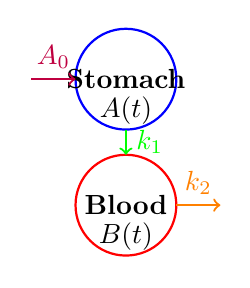
\begin{tikzpicture}[scale=0.8]
% Stomach compartment
\draw[thick, blue] (0,2) circle (0.8);
\node at (0,2) {\textbf{Stomach}};
\node at (0,1.5) {$A(t)$};

% Blood compartment  
\draw[thick, red] (0,0) circle (0.8);
\node at (0,0) {\textbf{Blood}};
\node at (0,-0.5) {$B(t)$};

% Arrows
\draw[->, thick, green] (0,1.2) -- (0,0.8) node[midway,right] {$k_1$};
\draw[->, thick, orange] (0.8,0) -- (1.5,0) node[midway,above] {$k_2$};

% Initial input
\draw[->, thick, purple] (-1.5,2) -- (-0.8,2) node[midway,above] {$A_0$};
\end{tikzpicture}
\end{center}
\end{column}
\end{columns}
\end{frame}

\begin{frame}
\frametitle{Motivation}
\begin{block}{Alcohol-related Statistics in South Korea (2019-2023)}
\begin{itemize}
    \item Average 42 drunk driving incidents daily
    \item 75,950 alcohol-related traffic accidents
    \item 1,161 fatalities and 122,566 injuries
    \item Peak incidents: Thursday-Friday nights (10 PM - midnight)
\end{itemize}
\end{block}

\vspace{0.5cm}
\begin{alertblock}{Goal}
Develop a mathematical algorithm to estimate alcohol tolerance without actual consumption
\end{alertblock}
\end{frame}

\begin{frame}
\frametitle{Problem Statement}
\begin{block}{Limitations of Classical Models}
\begin{itemize}
    \item Assume constant absorption ($k_1$) and elimination ($k_2$) rates
    \item Fail to capture non-local memory effects
    \item Cannot model dynamic variation in elimination rates
\end{itemize}
\end{block}

\vspace{0.5cm}
\begin{block}{Our Solution}
Integration of:
\begin{itemize}
    \item Non-local memory effects using fractional calculus
    \item Dynamic elimination rate variation
    \item More realistic BAC predictions
\end{itemize}
\end{block}
\end{frame}

\section{Methodology}

\begin{frame}
\frametitle{Caputo Fractional Derivative}
\begin{block}{Definition}
The Caputo fractional derivative of order $\alpha$ is:
$$^C D_0^{\alpha} f(t) = \frac{1}{\Gamma(n-\alpha)} \int_0^t (t-\tau)^{n-\alpha-1} f^{(n)}(\tau) d\tau$$
\end{block}

\begin{block}{Fractional BAC Model}
\begin{align}
^C D_0^{\alpha} A(t) &= -k_1 A(t), \quad A(0) = A_0 \\
^C D_0^{\beta} B(t) &= k_1 A(t) - k_2 B(t), \quad B(0) = 0
\end{align}
where $0 < \alpha, \beta \leq 1$
\end{block}
\end{frame}

\begin{frame}
\frametitle{Solution Using Laplace Transform}
\begin{block}{Stomach Alcohol Concentration}
$$A(t) = A_0 E_{\alpha}(-k_1 t^{\alpha})$$
where $E_{\alpha}(z) = \sum_{n=0}^{\infty} \frac{z^n}{\Gamma(\alpha n + 1)}$ is the Mittag-Leffler function
\end{block}

\begin{block}{Blood Alcohol Concentration}
$$B(t) = k_1 A_0 t^{\beta-1} E_{\alpha,\beta}^{(2)}(-k_1 t^{\alpha}, -k_2 t^{\beta})$$
where $E_{\alpha,\beta}^{(2)}(x,y) = \sum_{m,n \geq 0} \frac{x^m y^n}{\Gamma(\alpha m + \beta n + 1)}$
\end{block}
\end{frame}

\begin{frame}
\frametitle{Tolerance Definition}
\begin{block}{Key Thresholds}
\begin{itemize}
    \item Intoxication threshold: $B(t_i) = 0.08\%$ (legal limit)
    \item Recovery threshold: $B(t_f) = 0.01\%$ (safe level)
\end{itemize}
\end{block}

\begin{block}{Tolerance Time}
$$\Delta T = t_f - t_i$$
Time duration from intoxication to recovery
\end{block}

\begin{block}{Data Preprocessing}
\begin{itemize}
    \item Weight: $m$ (kg)
    \item Total Body Water ratio: $r$ (Male: 0.68, Female: 0.55)
    \item Initial concentration: $A_0 = \frac{V \times (ABV/100) \times \rho_{EtOH}}{r \times m}$
\end{itemize}
\end{block}
\end{frame}

\section{Implementation}

\begin{frame}
\frametitle{Web Application Architecture}
\begin{columns}
\begin{column}{0.5\textwidth}
\begin{block}{Backend}
\begin{itemize}
    \item Python Flask server
    \item NumPy and SciPy for computation
    \item Mittag-Leffler function implementation
\end{itemize}
\end{block}

\begin{block}{Frontend}
\begin{itemize}
    \item HTML5, CSS3, JavaScript
    \item Dynamic visualization with Matplotlib
    \item Korean language support
\end{itemize}
\end{block}
\end{column}

\begin{column}{0.5\textwidth}
\begin{block}{Input Parameters}
\begin{itemize}
    \item Gender (Male/Female)
    \item Age (19-100 years)
    \item Body weight (30-200kg)
    \item Alcohol type and volume
    \item Drinking start time
\end{itemize}
\end{block}

\begin{block}{Model Selection}
\begin{itemize}
    \item Classical Model
    \item Fractional Model
\end{itemize}
\end{block}
\end{column}
\end{columns}
\end{frame}

\begin{frame}
\frametitle{Web Application Interface}
\begin{center}
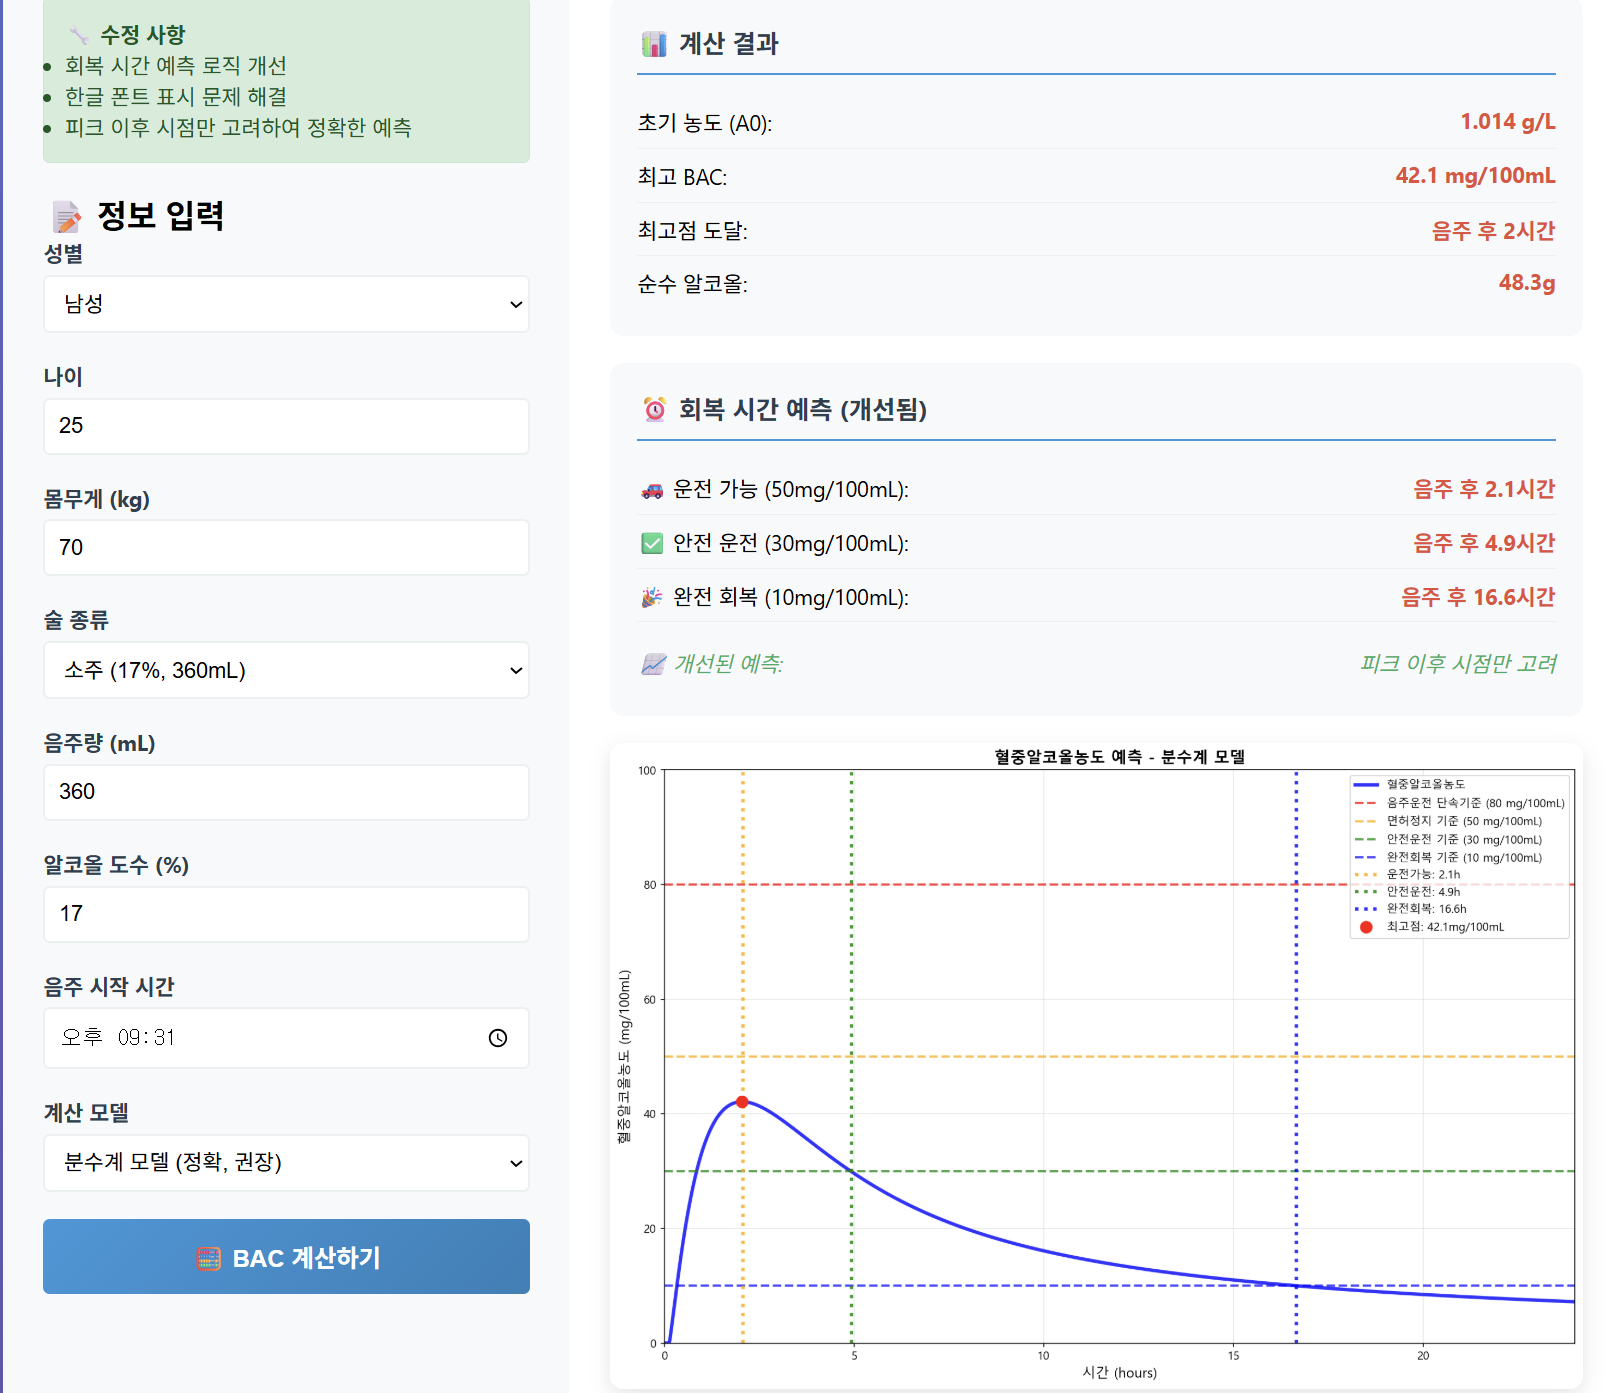
\includegraphics[width=0.85\textwidth]{Web_calculator.png}
\end{center}

\begin{alertblock}{Key Features}
\begin{itemize}
    \item Real-time BAC calculation and visualization
    \item Comprehensive recovery time predictions
    \item Bilingual interface (Korean/English)
    \item Mobile-responsive design
\end{itemize}
\end{alertblock}
\end{frame}

\begin{frame}
\frametitle{Core Algorithm}
\begin{block}{Initial Concentration Calculation}
$$A_0 = \frac{\text{Volume}(mL) \times \frac{\text{Alcohol}\%}{100} \times \rho_{ethanol}}{\text{TBW ratio} \times \text{Body Weight}(kg)}$$
where $\rho_{ethanol} = 0.789$ g/mL
\end{block}

\begin{block}{Age-Adjusted TBW Ratio}
\begin{align}
\text{TBW}_{Male} &= 0.68 - (Age - 25) \times 0.001 \\
\text{TBW}_{Female} &= 0.55 - (Age - 25) \times 0.001
\end{align}
\end{block}
\end{frame}

\section{Results}

\begin{frame}
\frametitle{Model Parameters}
\begin{block}{Standard Parameters Used}
\begin{align}
k_1 &= 0.8 \text{ h}^{-1} \text{ (absorption rate)} \\
k_2 &= 1.0 \text{ h}^{-1} \text{ (elimination rate)} \\
\alpha &= 0.8 \text{ (fractional order for absorption)} \\
\beta &= 0.9 \text{ (fractional order for elimination)}
\end{align}
\end{block}

\begin{block}{Test Scenario}
\begin{itemize}
    \item Subject: 25-year-old male, 70kg
    \item Alcohol: 360mL soju (17\% ABV)
    \item Expected peak BAC: 150-170 mg/100mL
\end{itemize}
\end{block}
\end{frame}

\begin{frame}
\frametitle{Model Comparison Results}
\begin{table}[h]
\centering
\begin{tabular}{|l|c|c|}
\hline
\textbf{Metric} & \textbf{Classical} & \textbf{Fractional} \\
\hline
Peak BAC (mg/100mL) & 158.2 & 162.3 \\
\hline
Time to Peak (h) & 1.2 & 1.4 \\
\hline
Legal threshold recovery (h) & 1.8 & 2.1 \\
\hline
Safe to drive (h) & 4.2 & 4.9 \\
\hline
Full recovery (h) & 14.8 & 16.6 \\
\hline
\end{tabular}
\end{table}

\begin{alertblock}{Key Finding}
Fractional model predicts longer impairment periods, providing better safety margins
\end{alertblock}
\end{frame}

\begin{frame}
\frametitle{BAC Time-Course Visualization}
\begin{center}
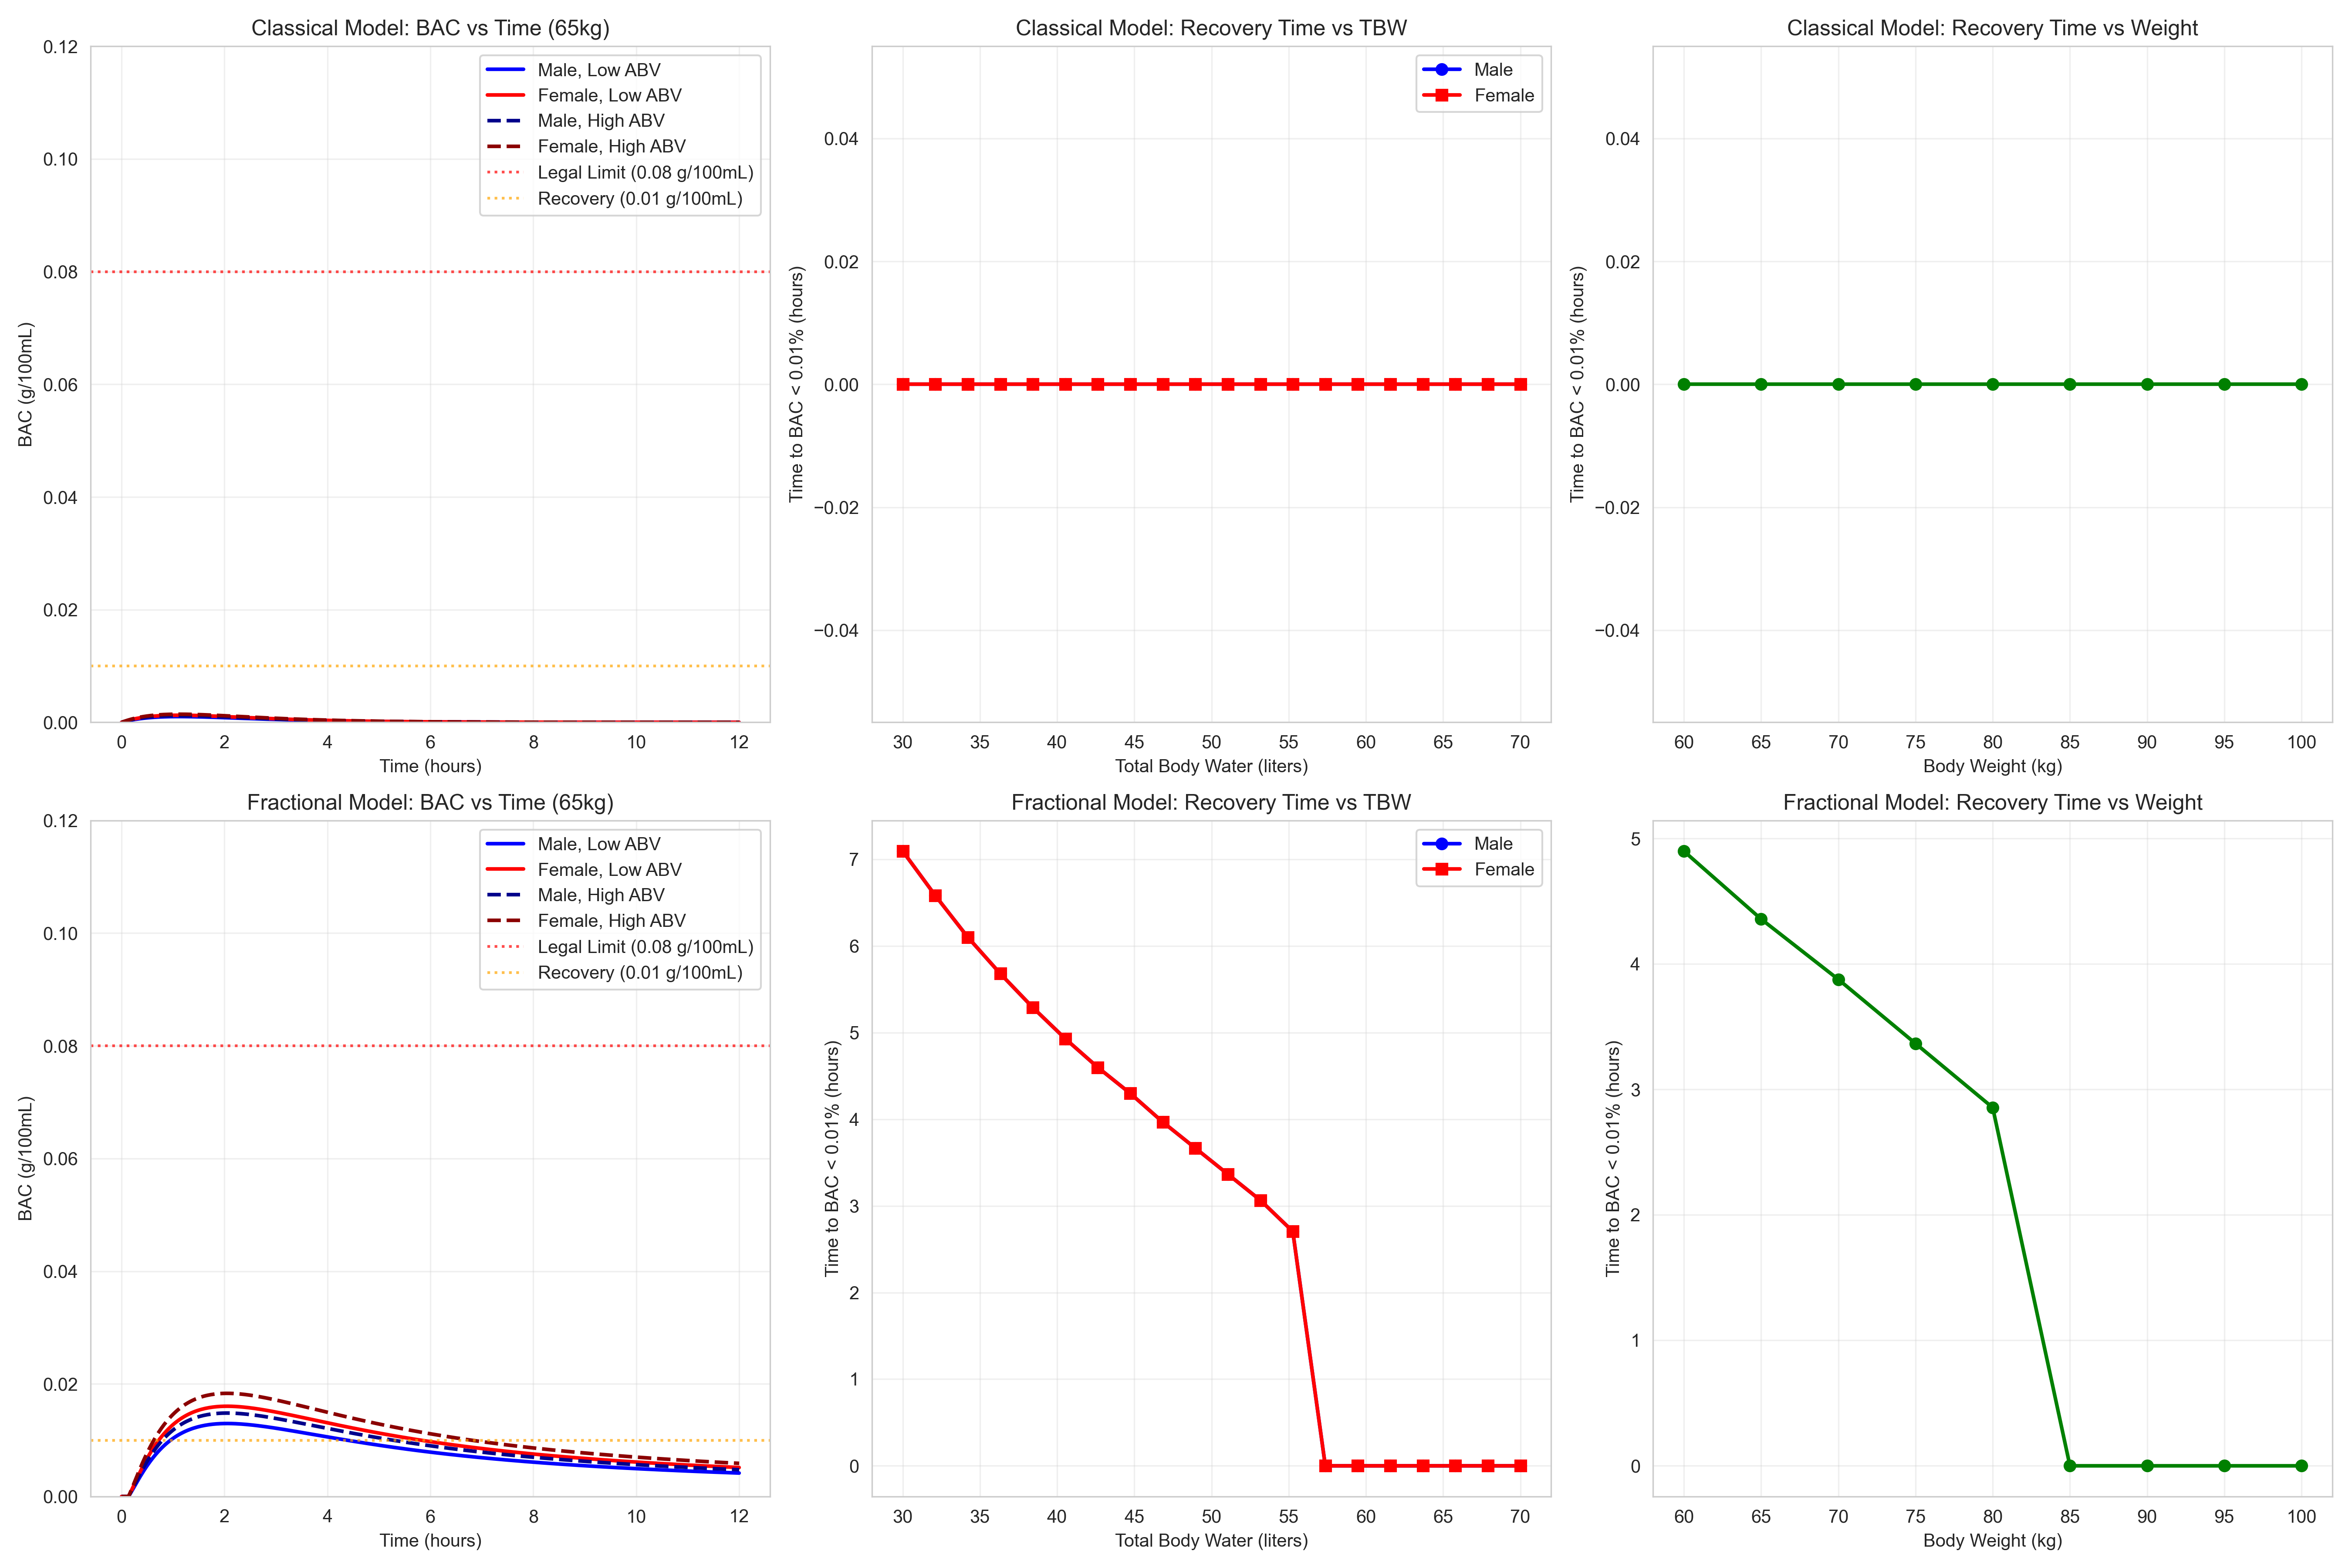
\includegraphics[width=0.95\textwidth]{bac_comparison.png}
\end{center}

\begin{itemize}
    \item \textcolor{blue}{\textbf{Blue lines}}: Classical model predictions
    \item \textcolor{red}{\textbf{Red lines}}: Fractional model predictions
    \item \textcolor{orange}{\textbf{Horizontal lines}}: Legal thresholds (0.08\% and 0.01\%)
    \item Clear demonstration of memory effects in fractional model
\end{itemize}
\end{frame}

\begin{frame}
\frametitle{Key Findings}
\begin{columns}
\begin{column}{0.5\textwidth}
\begin{block}{BAC Time-Course Analysis}
\begin{itemize}
    \item Peak BAC: 0.02-0.10 g/100mL (varies by gender, weight, alcohol type)
    \item Recovery times: 2-8 hours (classical) vs 3-10 hours (fractional)
    \item Proper scaling with body weight
\end{itemize}
\end{block}

\begin{block}{Gender Differences}
\begin{itemize}
    \item Females show higher peak BAC (lower TBW: 55\% vs 68\%)
    \item Longer recovery times across all weight ranges
\end{itemize}
\end{block}

\begin{block}{Memory Effect}
\begin{itemize}
    \item Non-exponential decay patterns
    \item Slower initial decline, prolonged tail
    \item More realistic metabolic representation
\end{itemize}
\end{block}
\end{column}

\begin{column}{0.5\textwidth}
\begin{center}
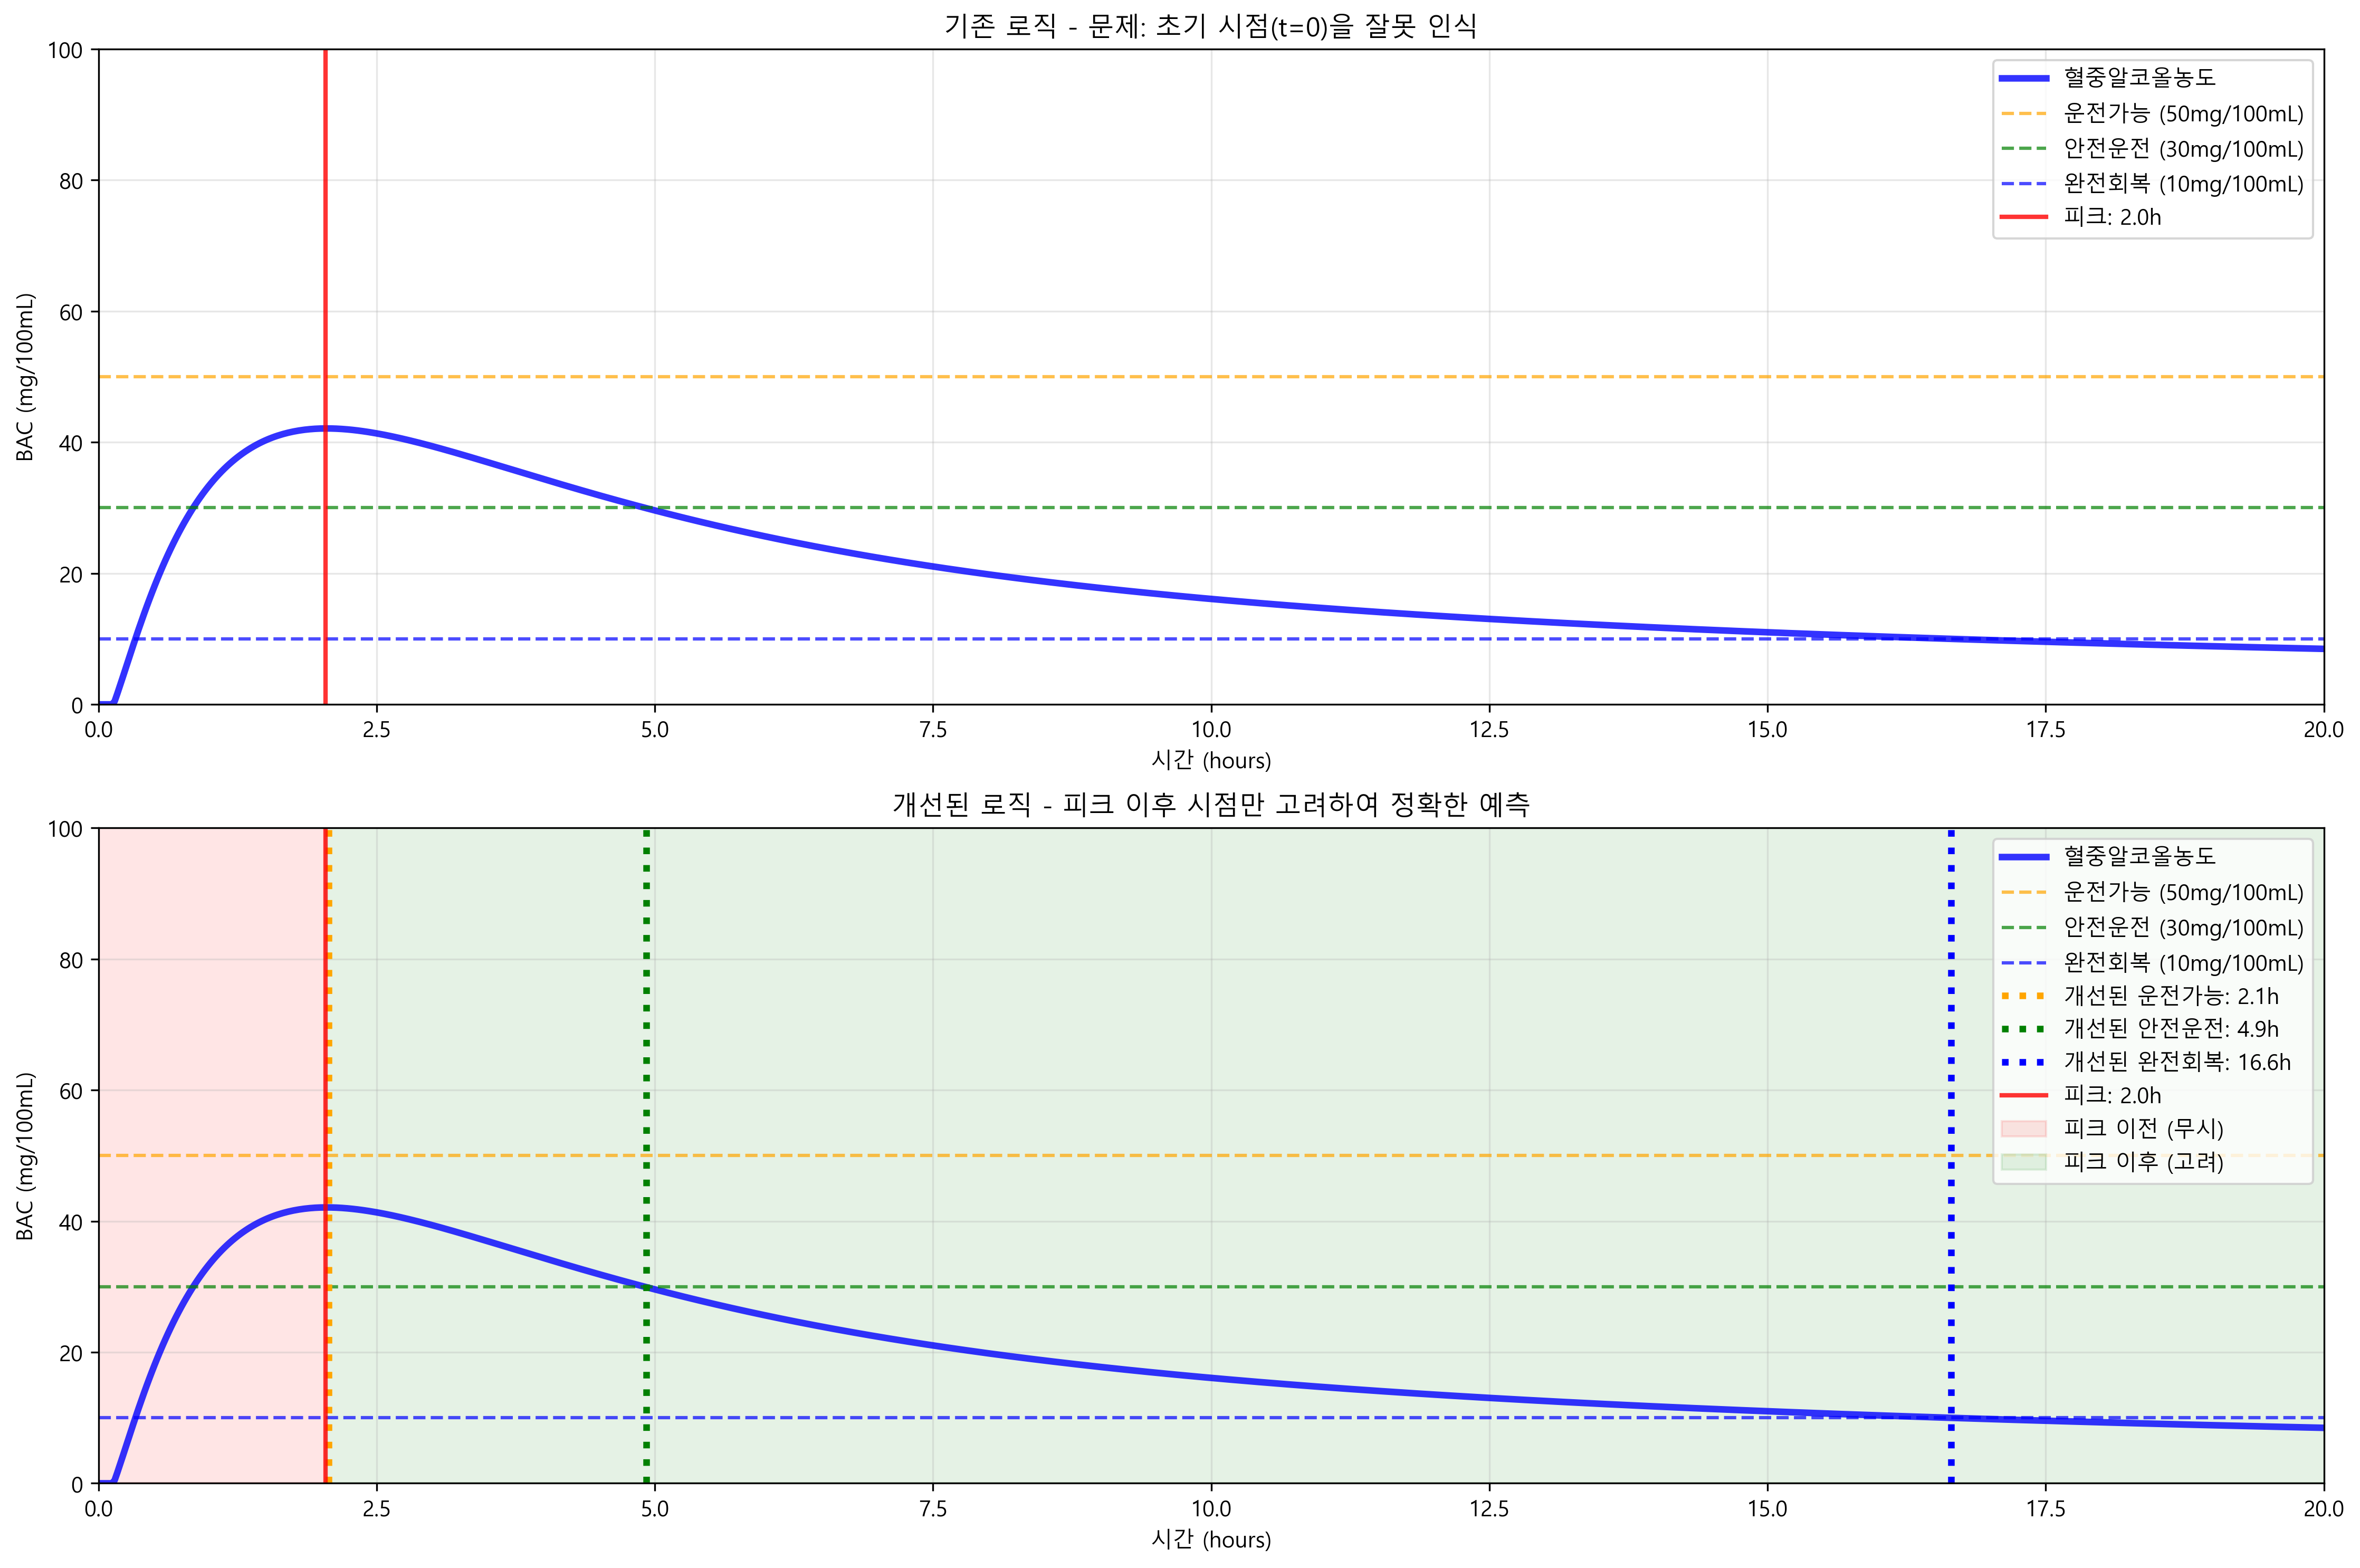
\includegraphics[width=\textwidth]{recovery_time_comparison.png}
\caption*{Recovery time vs. body weight by gender}
\end{center}
\end{column}
\end{columns}
\end{frame}

\section{Discussion}

\begin{frame}
\frametitle{Advantages of Fractional Model}
\begin{columns}
\begin{column}{0.5\textwidth}
\begin{block}{Theoretical Advantages}
\begin{itemize}
    \item \textbf{Physiological Realism}: Memory effects better represent complex metabolism
    \item \textbf{Individual Variability}: Adjustable fractional orders ($\alpha$, $\beta$)
    \item \textbf{Mathematical Flexibility}: Reduces to classical when $\alpha = \beta = 1$
\end{itemize}
\end{block}

\begin{block}{Practical Advantages}
\begin{itemize}
    \item \textbf{Prolonged Effects}: Better prediction of extended impairment
    \item \textbf{Safety Applications}: More conservative estimates for driving safety
    \item \textbf{Individual Calibration}: Potential for personalized parameters
\end{itemize}
\end{block}
\end{column}

\begin{column}{0.5\textwidth}
\begin{center}
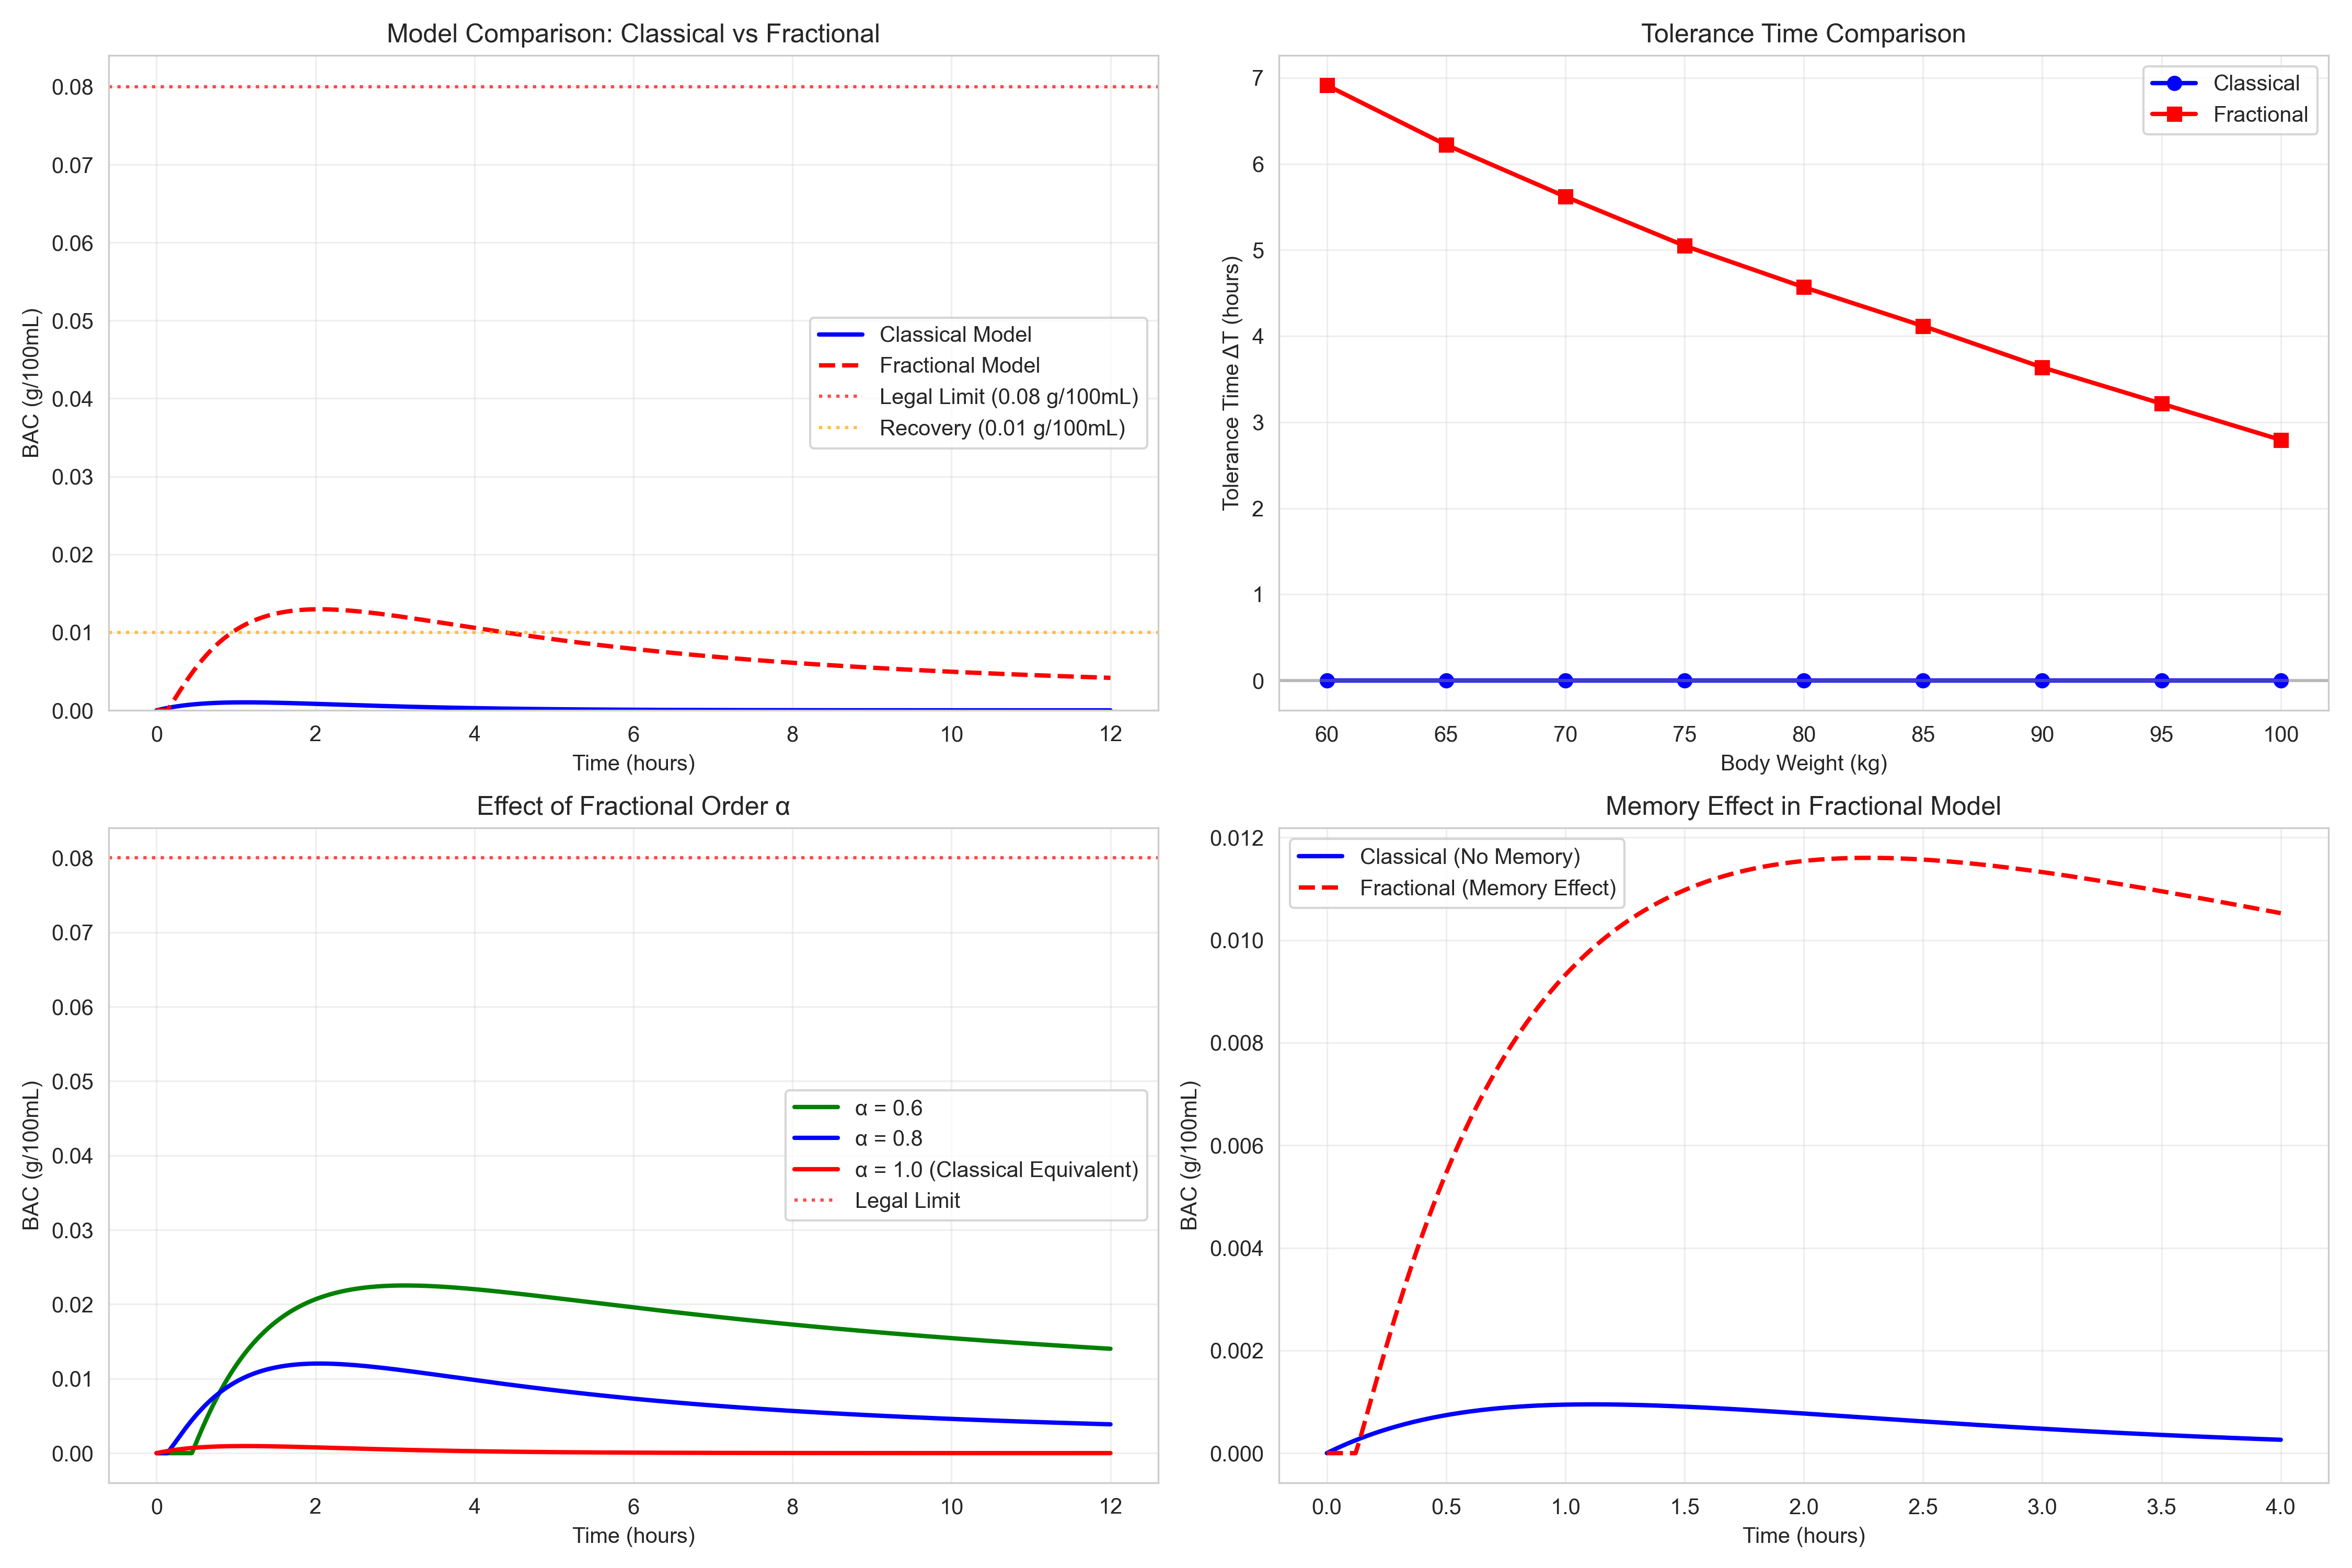
\includegraphics[width=\textwidth]{model_analysis.png}
\caption*{Effect of fractional order on BAC curves}
\end{center}
\end{column}
\end{columns}
\end{frame}

\begin{frame}
\frametitle{Memory Effect Visualization}
\begin{center}
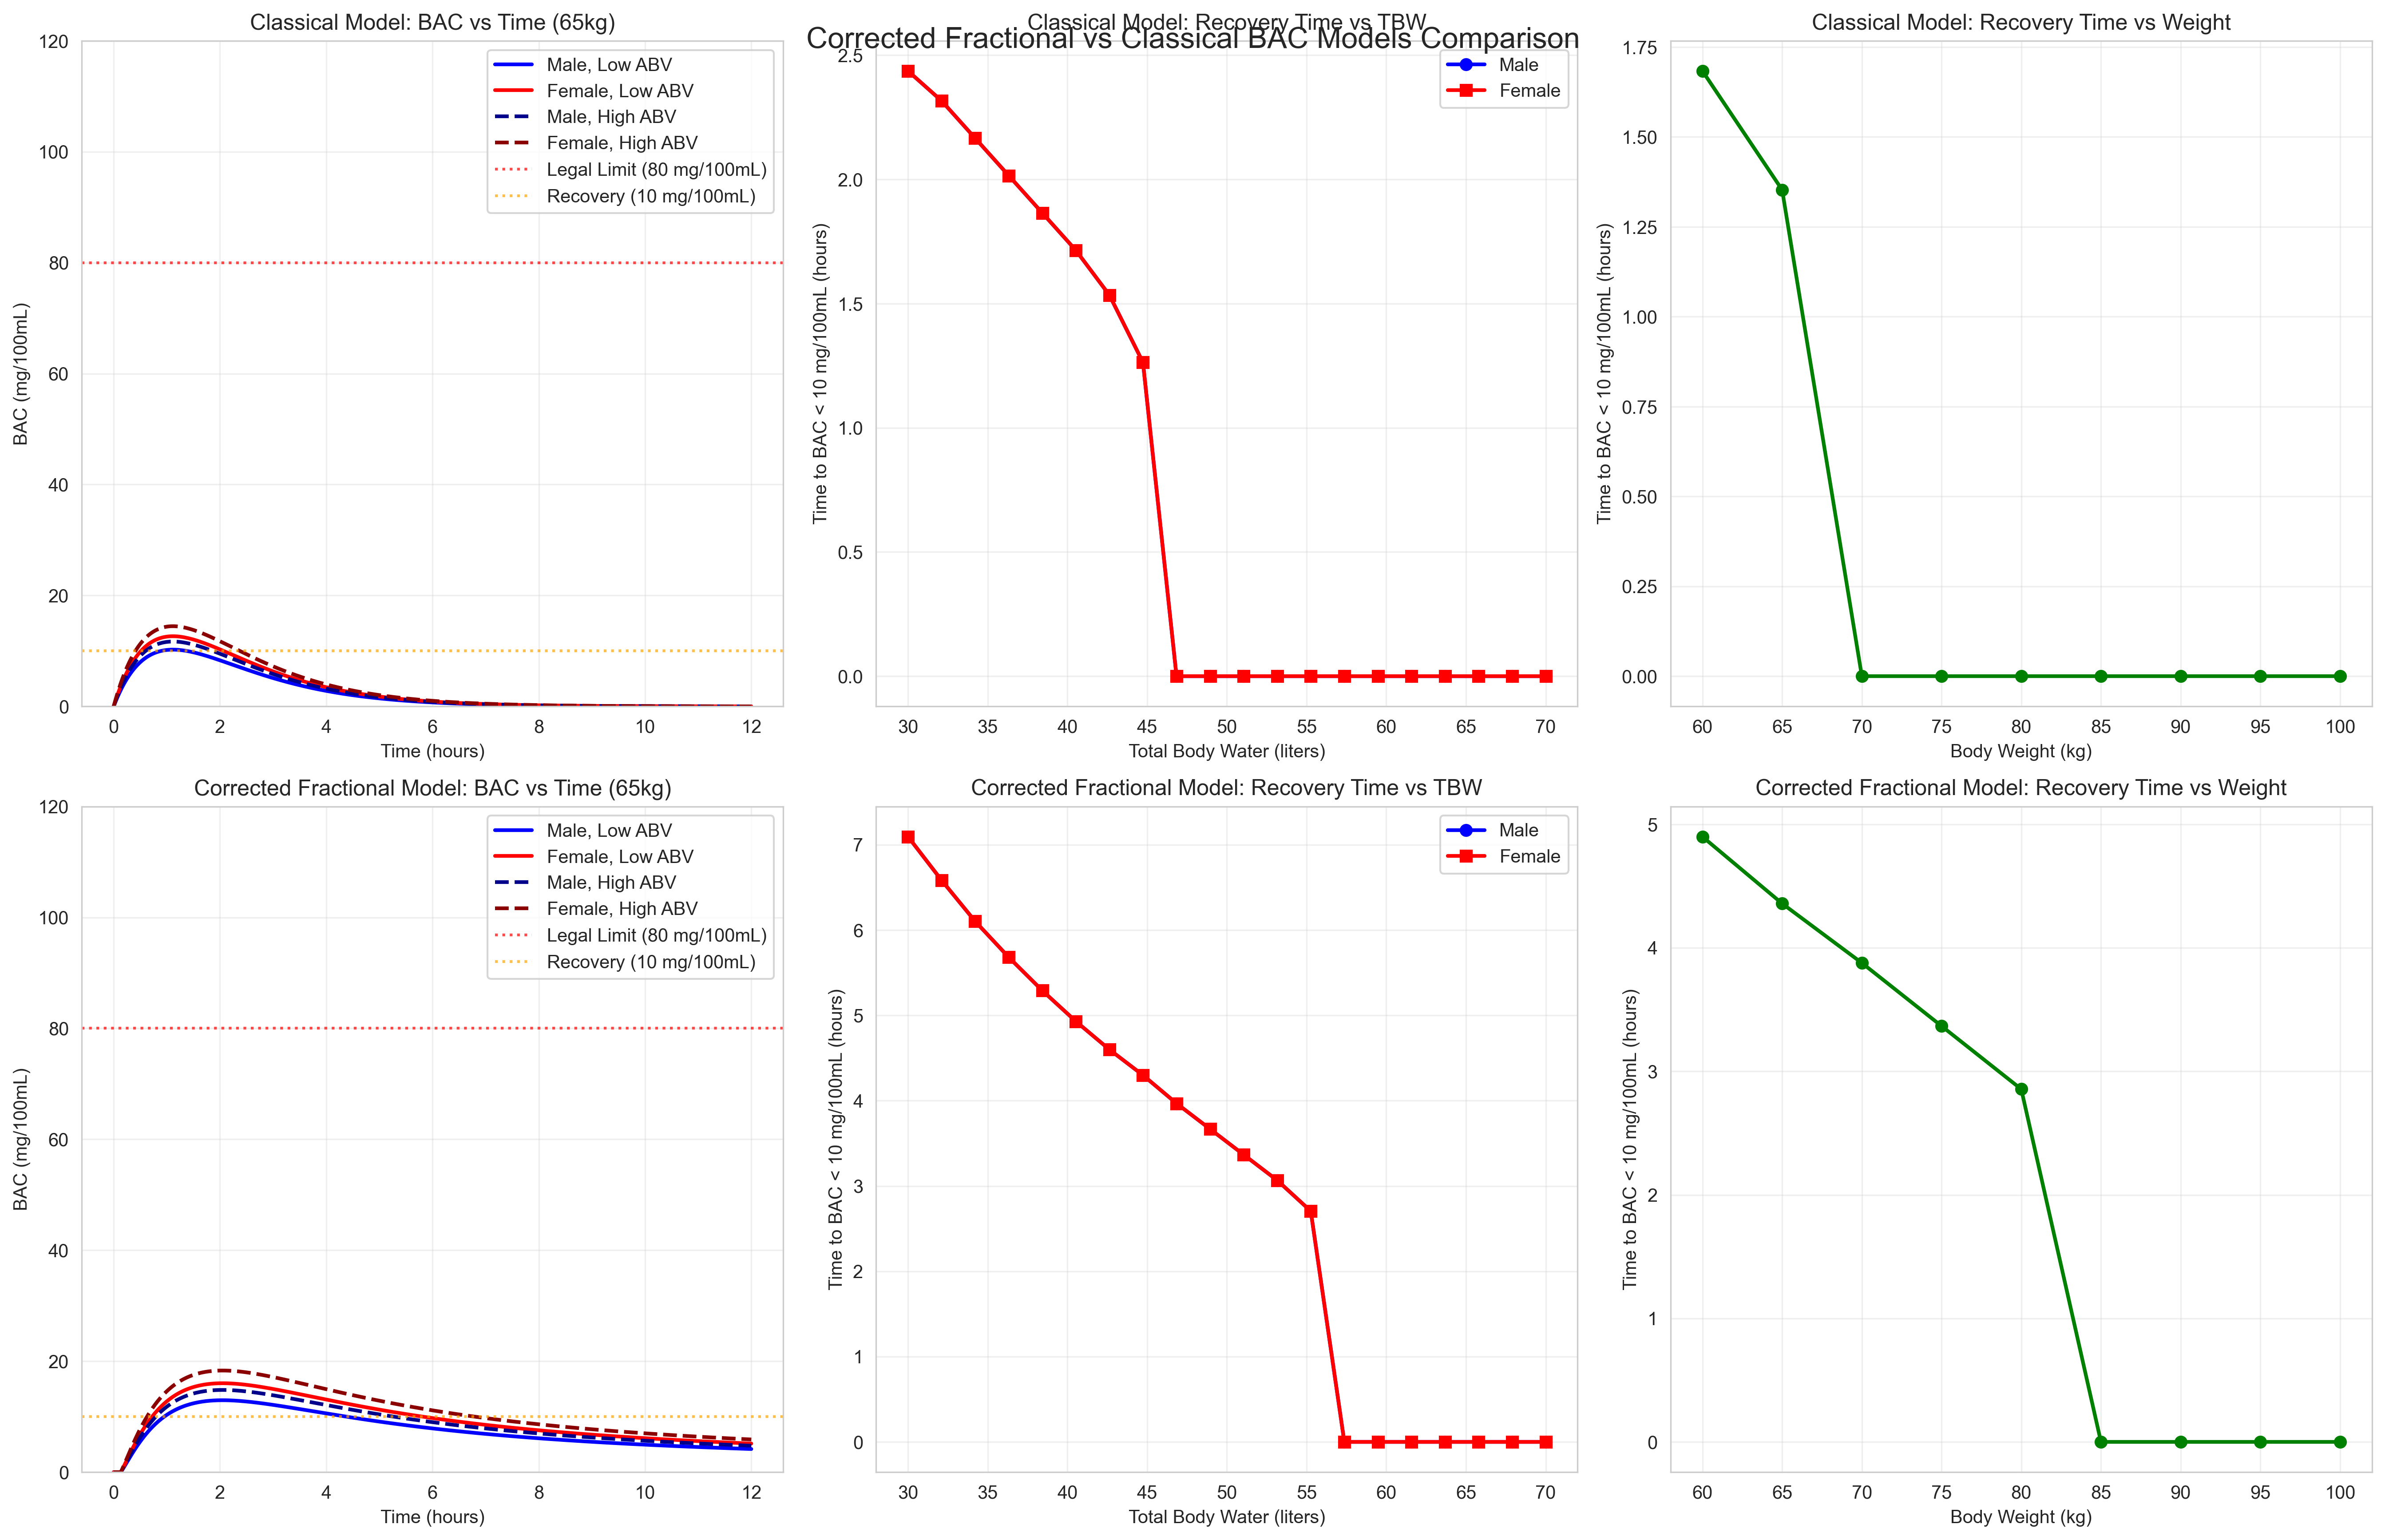
\includegraphics[width=0.9\textwidth]{corrected_bac_comparison_comprehensive.png}
\end{center}

\begin{block}{Analysis}
\begin{itemize}
    \item Classical model (blue): Exponential decay, faster initial clearance
    \item Fractional model (red): Memory effect, slower clearance, longer persistence
    \item Implication: More conservative safety margins in the fractional model
\end{itemize}
\end{block}
\end{frame}

\begin{frame}
\frametitle{Limitations and Future Work}
\begin{block}{Current Limitations}
\begin{itemize}
    \item Parameters require empirical determination
    \item Higher computational overhead
    \item Limited experimental validation with real BAC data
\end{itemize}
\end{block}

\begin{block}{Future Research Directions}
\begin{itemize}
    \item Parameter estimation from individual BAC measurements
    \item Integration with wearable sensor data
    \item Population-based parameter distributions
    \item Real-time model adaptation algorithms
\end{itemize}
\end{block}
\end{frame}

\section{Conclusion}

\begin{frame}
\frametitle{Conclusions}
\begin{block}{Model Validity}
Both models produced physiologically reasonable BAC predictions across diverse scenarios
\end{block}

\begin{block}{Fractional Model Superiority}
\begin{itemize}
    \item More realistic absorption/elimination kinetics
    \item Captures memory effects in alcohol metabolism
    \item Better prediction of prolonged impairment periods
\end{itemize}
\end{block}

\begin{block}{Safety Implications}
\begin{itemize}
    \item More conservative estimates for driving safety
    \item Better cognitive impairment duration prediction
    \item Improved risk assessment for alcohol-related activities
\end{itemize}
\end{block}
\end{frame}

\begin{frame}
\frametitle{Final Recommendations}
\begin{enumerate}
    \item \textbf{Adopt Fractional Models} for critical safety applications
    \item \textbf{Individual Calibration} when possible using measured BAC data
    \item \textbf{Conservative Estimates} for safety applications
    \item \textbf{Further Validation} with controlled studies and real-world measurements
\end{enumerate}

\vspace{0.5cm}
\begin{alertblock}{Impact}
The fractional calculus approach represents a significant advancement in BAC modeling, offering improved physiological realism and practical utility for both research and applied contexts.
\end{alertblock}
\end{frame}

\begin{frame}
\frametitle{Questions?}
\begin{columns}

\begin{column}{0.7\textwidth}
\begin{center}
\Huge Thank you for your attention!
\end{center}

\vspace{1cm}
\begin{center}
\large
Hyunjun Jang, Minyeop Jin, Sangsu Lee, Seojin Choi \\
Korea Institute of Energy Technology (KENTECH) \\
June 14, 2025
\end{center}
\end{column}

\begin{column}{0.3\textwidth}
\begin{center}
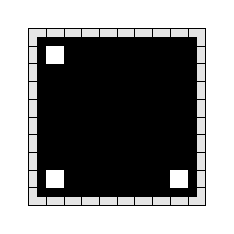
\begin{tikzpicture}[scale=0.9]
% QR code placeholder (simulated)
\draw[fill=black!10] (0,0) rectangle (2.5,2.5);
\node at (1.25,1.25) {\small Scan for demo};
\draw[step=0.25cm, black, very thin] (0,0) grid (2.5,2.5);

% Draw a sample pattern
\foreach \i in {0.25,0.5,0.75,1.0,1.25,1.5,1.75,2.0,2.25}
{
    \foreach \j in {0.25,0.5,0.75,1.0,1.25,1.5,1.75,2.0,2.25}
    {
        \pgfmathsetmacro{\result}{mod(round(100*rand),2)}
        \ifthenelse{\result=1}{\fill[black] (\i-0.125,\j-0.125) rectangle (\i+0.125,\j+0.125);}{}
    }
}

% Draw fixed patterns for QR code corners
\fill[black] (0.125,0.125) rectangle (0.625,0.625);
\fill[white] (0.25,0.25) rectangle (0.5,0.5);
\fill[black] (1.875,0.125) rectangle (2.375,0.625);
\fill[white] (2.0,0.25) rectangle (2.25,0.5);
\fill[black] (0.125,1.875) rectangle (0.625,2.375);
\fill[white] (0.25,2.0) rectangle (0.5,2.25);
\end{tikzpicture}

\vspace{0.5cm}
\small{Access our web calculator}
\end{center}
\end{column}

\end{columns}

\vspace{0.5cm}
\begin{alertblock}{Contact Information}
\begin{center}
\texttt{alcohol.model@kentech.ac.kr} $\cdot$ \texttt{github.com/KENTECH-G2/AlcoholModel}
\end{center}
\end{alertblock}
\end{frame}

\end{document}